\documentclass{beamer}
\usepackage{graphicx}
\title{Week 2 Presentation}
\author{Nick, Sriram, Rohit, Silas}
\begin{document}
    \maketitle
    \begin{frame}
        \frametitle{Tennis Tree Regression}

        Highlight of Tennis Grid Search Model Comparison
        \newline
        \resizebox{\textwidth}{!}{
            \begin{tabular}{l|r|r|r|r|r|r}
            \hline
            comment & cp & minsplit & maxdepth & train\_error & test\_error & nsplits\\
            \hline
            least test error & 0.000 & 2 & 1 & 0.229 & 0.277 & 1\\
            \hline
            reasonable performer using more than one split & 0.001 & 40 & 5 & 0.224 & 0.279 & 6\\
            \hline
            worst overfit & 0.000 & 2 & 15 & 0.079 & 0.345 & 434\\
            \hline
            \end{tabular}
        }
        \newline

        Best model: 
        \begin{columns}[c]
            \begin{column}{0.4\textwidth}
                \centering
                
\includegraphics[height=.7\textwidth]{plots/tennis_mod_winner_rpart_plot.png}
                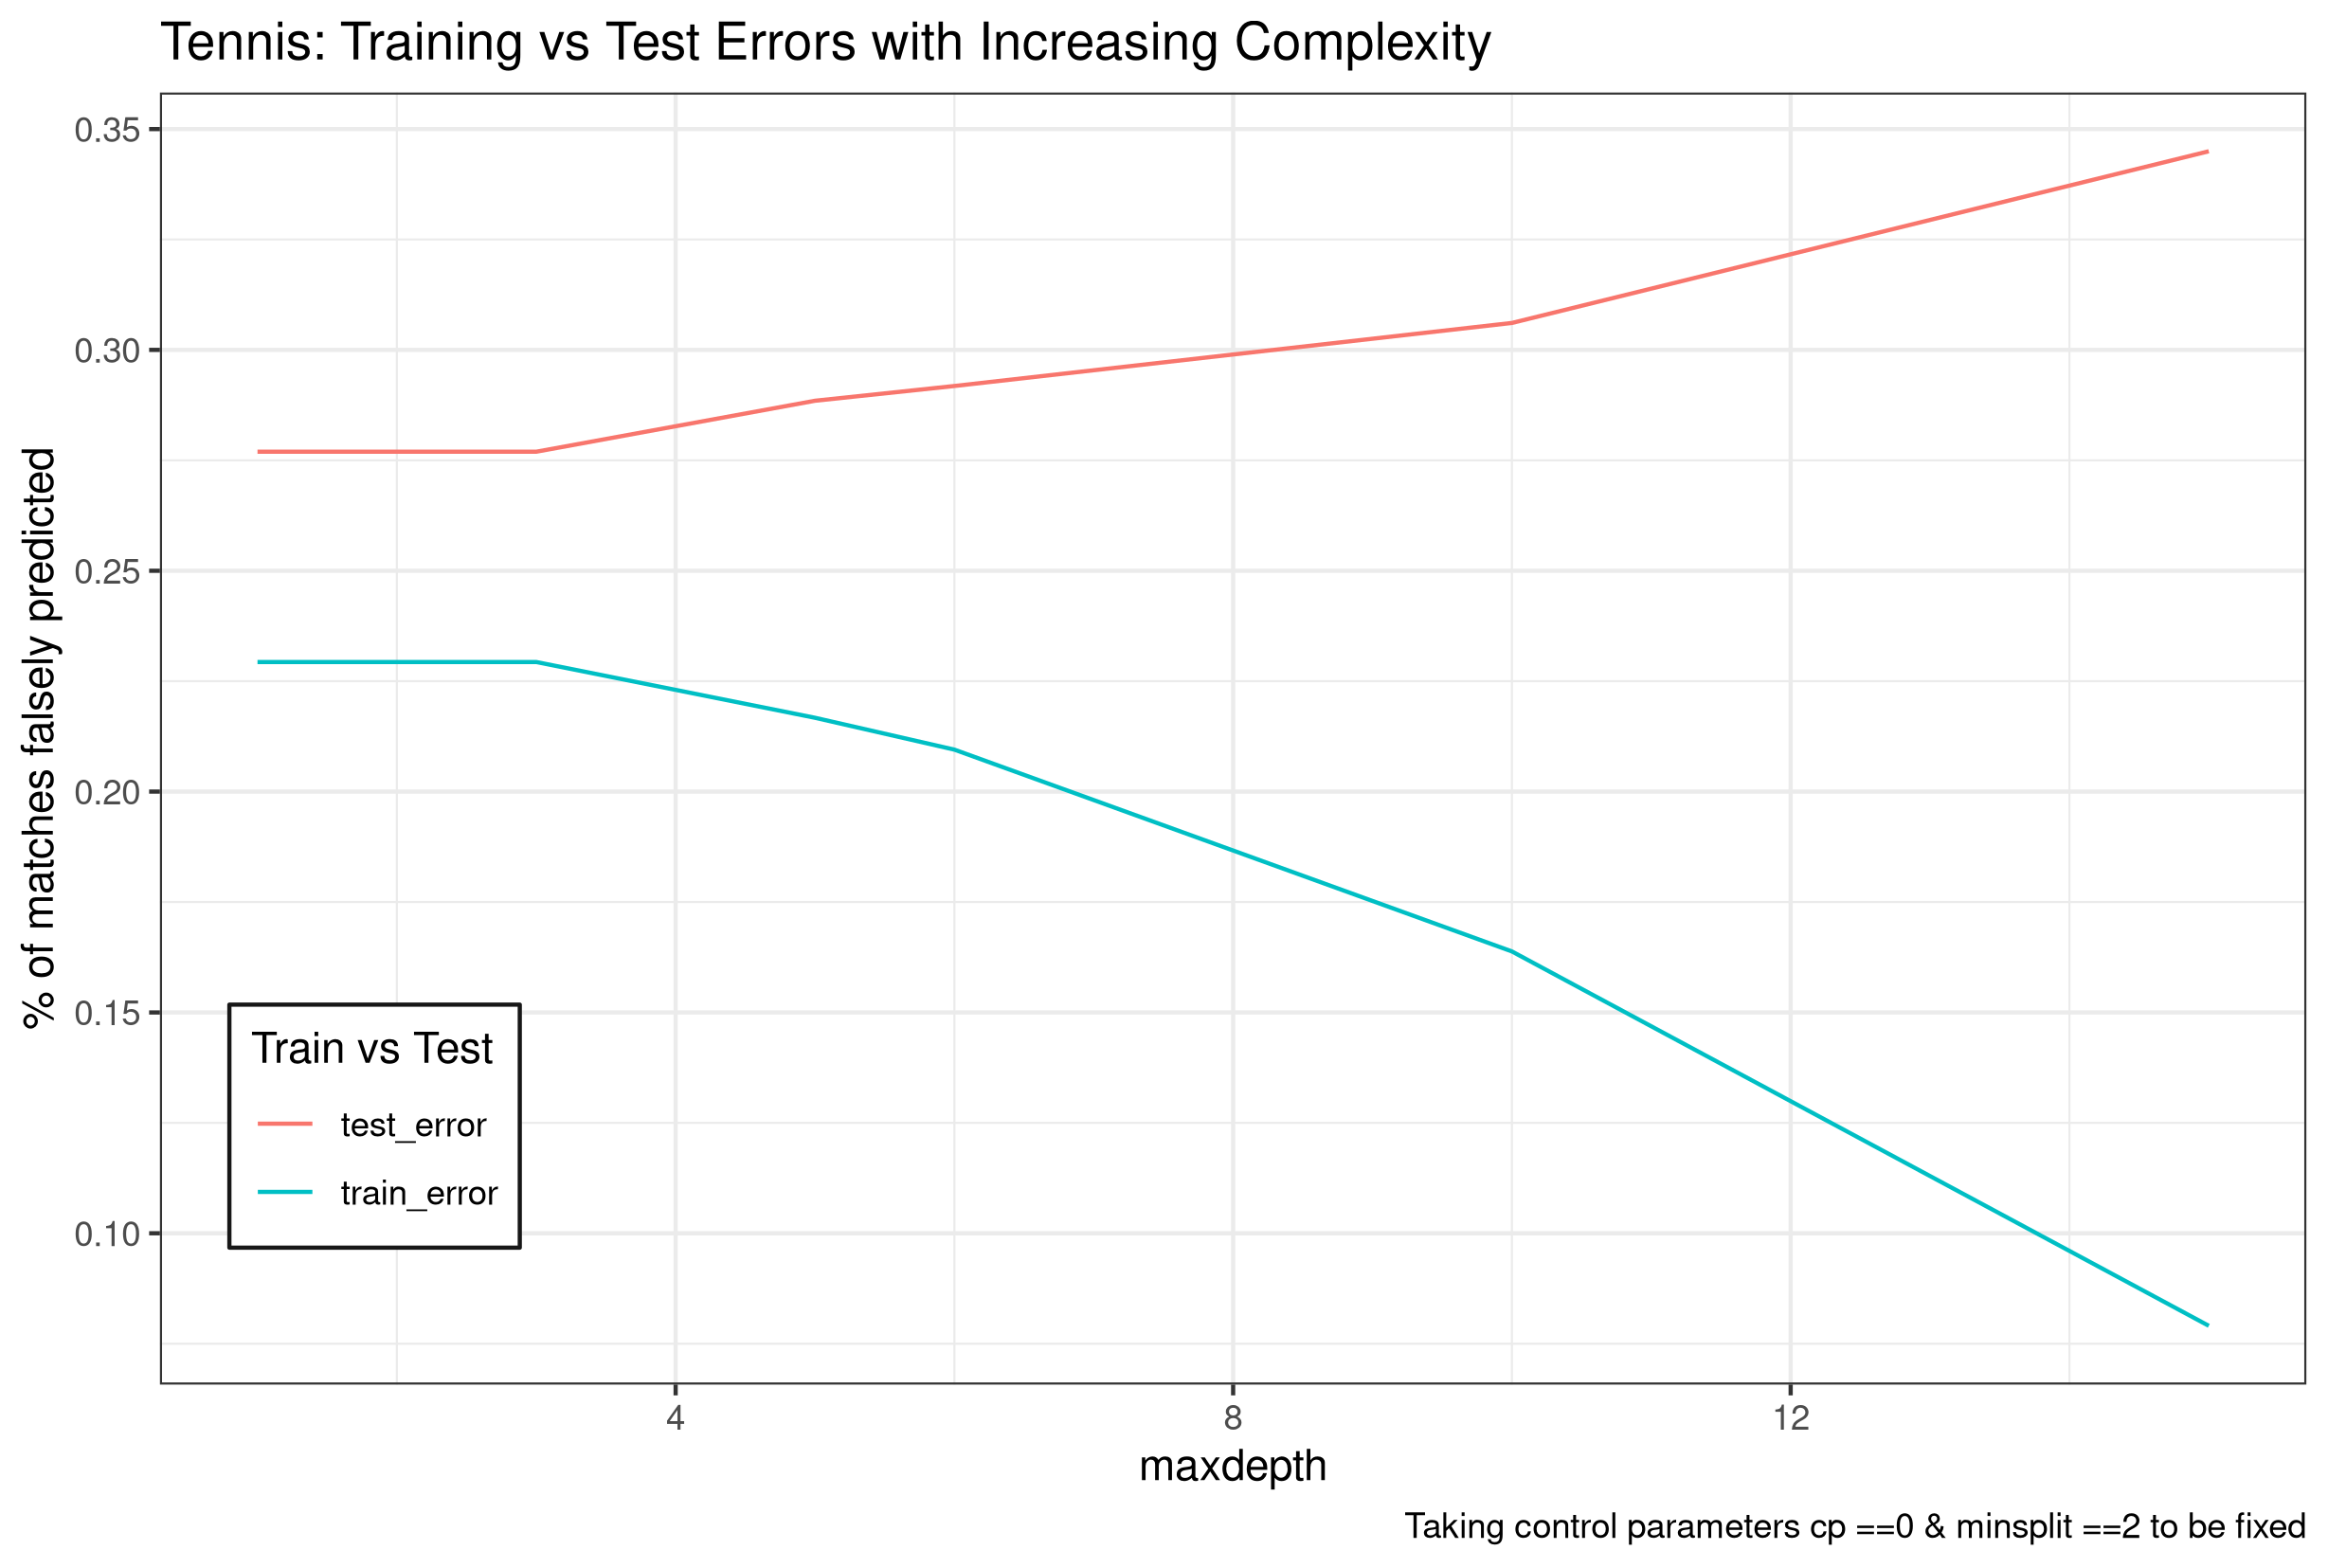
\includegraphics[width=\textwidth]{plots/tennis_overfit_complexity.png}
            \end{column}
            \begin{column}{0.6\textwidth}
                \newline
                \centering
                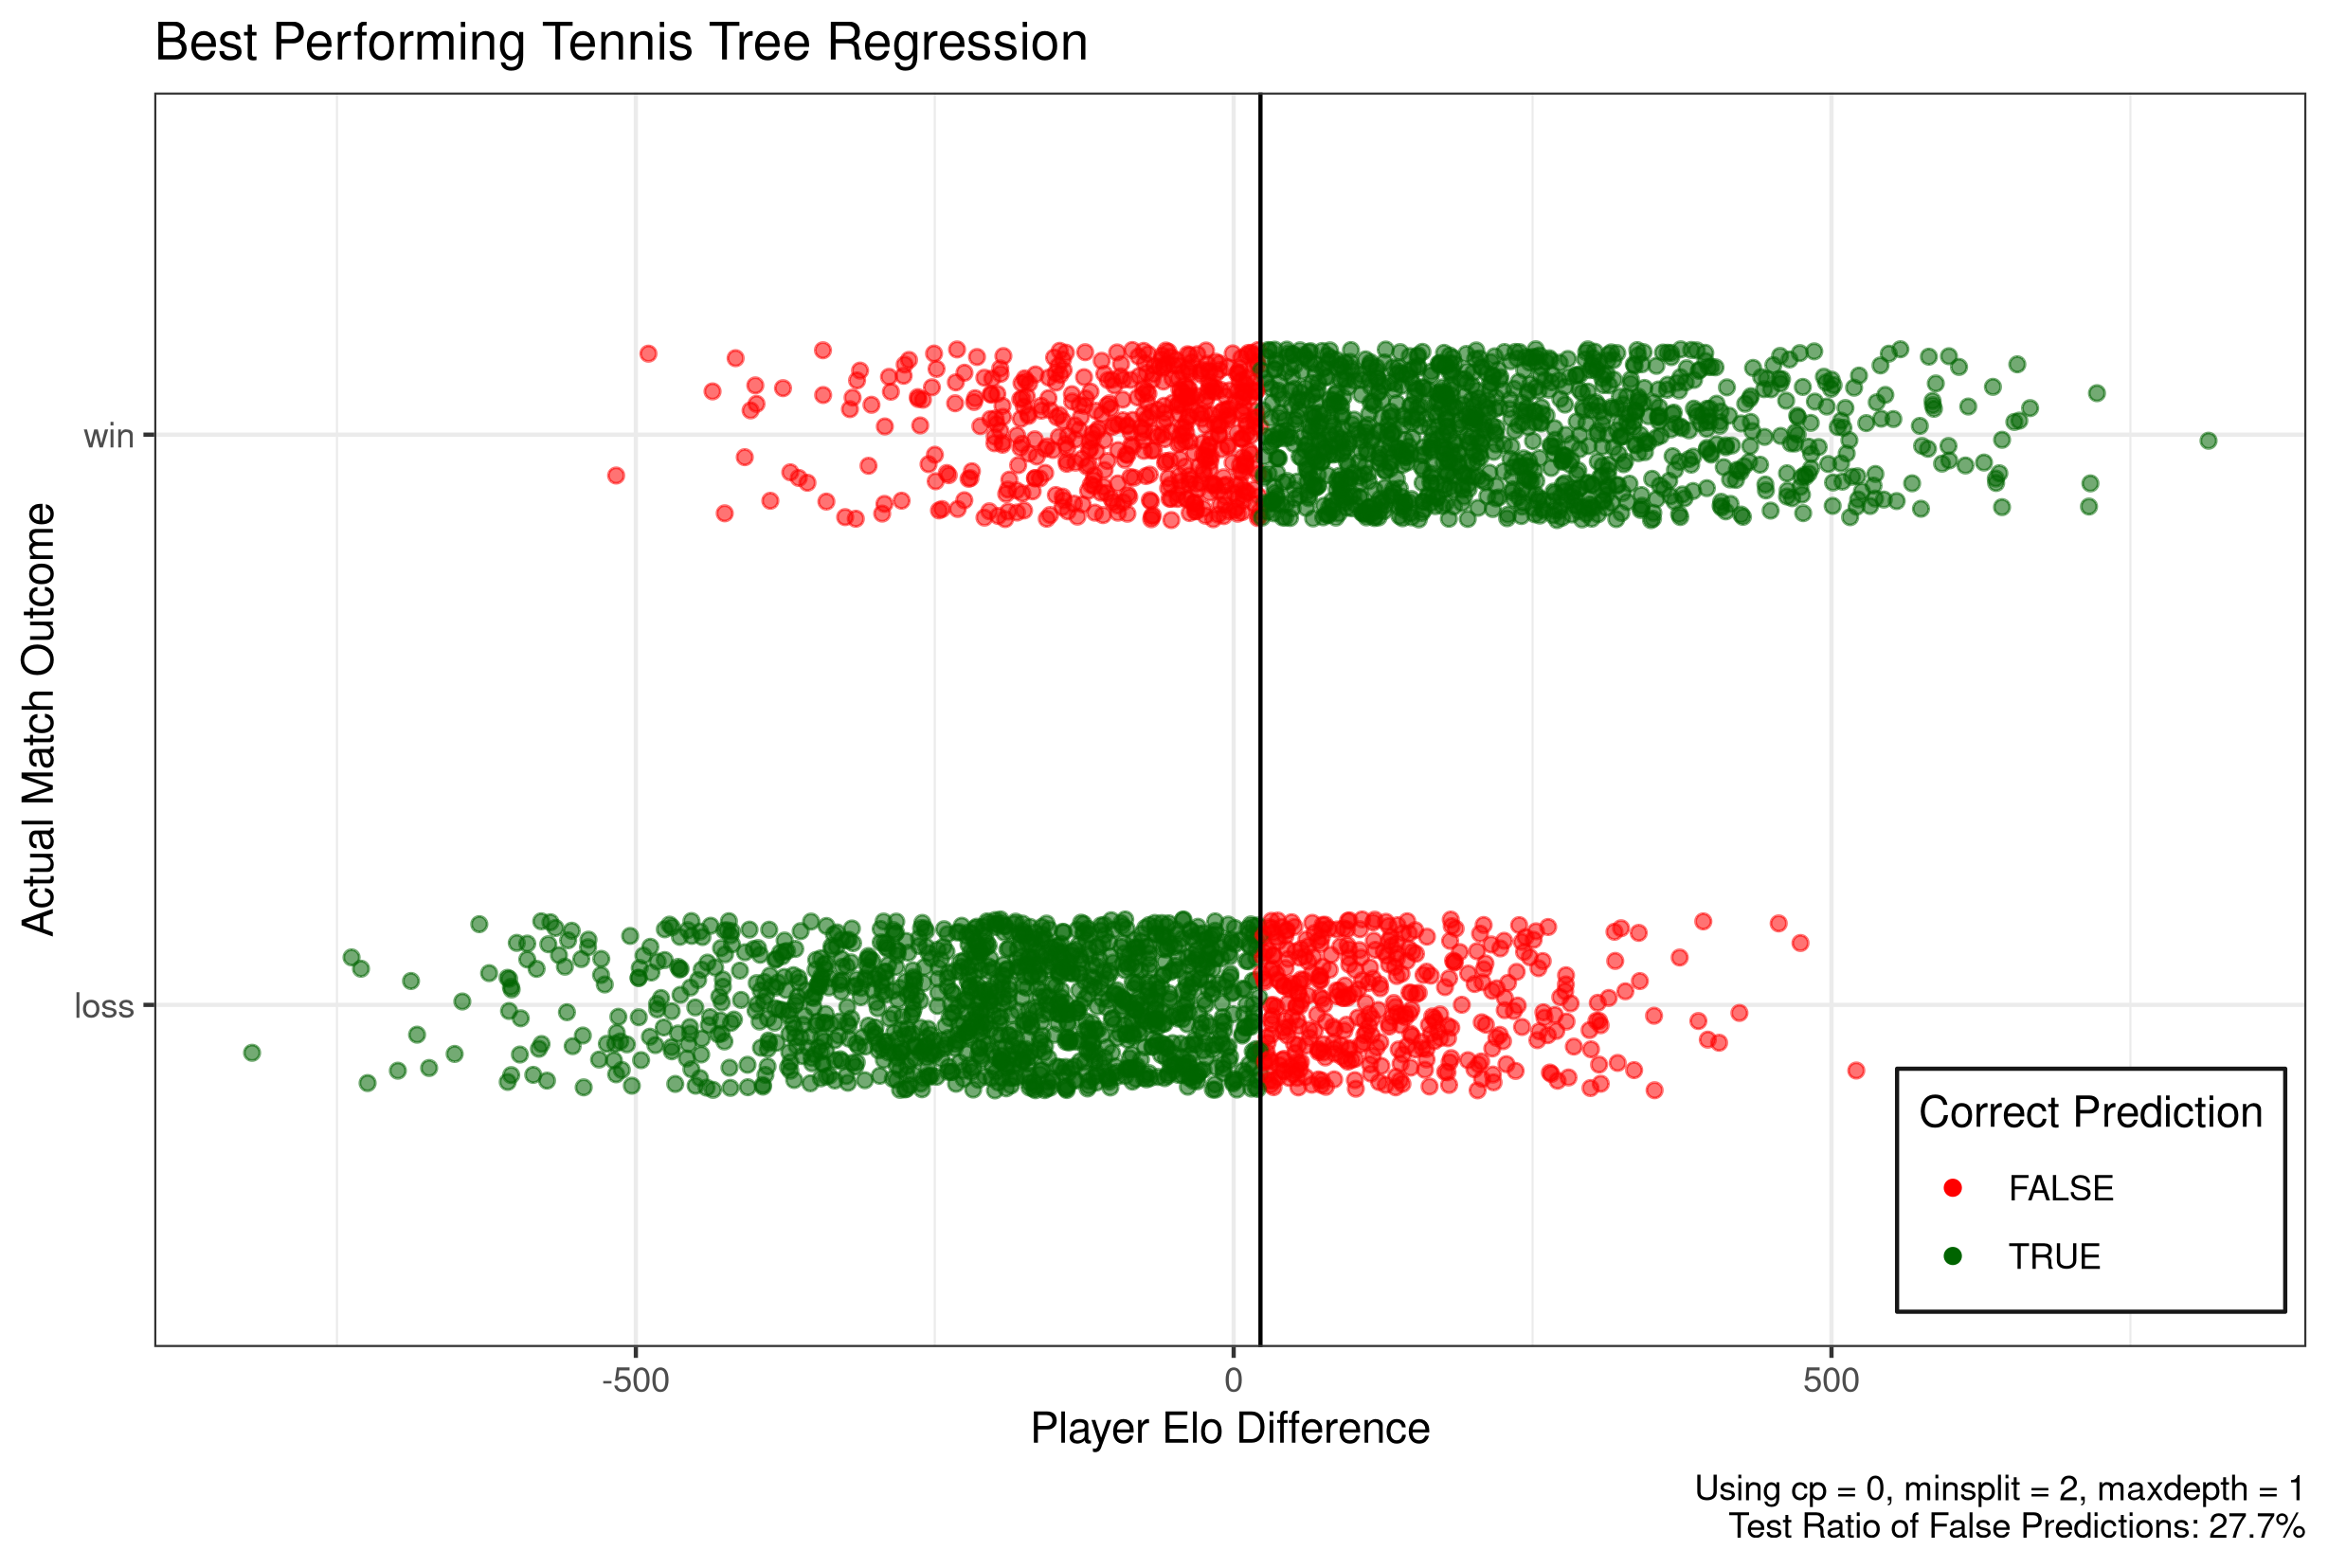
\includegraphics[width=\textwidth]{plots/tennis_best_tree_scatter.png}
            \end{column}
        \end{columns}
    \end{frame}


    \begin{frame}
        \frametitle{Handball Tree Regression}

        Highlight of Handball Grid Search Model Comparison
        \newline
        \resizebox{\textwidth}{!} {
            \begin{tabular}{l|r|r|r|r|r|r|r|r}
            \hline
            comment & cp & minsplit & maxdepth & train\_mae & train\_rmse & test\_mae & test\_rmse & nsplits\\
            \hline
            best test mae & 0 & 40 & 5 & 3.288 & 4.213 & 3.588 & 4.582 & 25\\
            \hline
            compromise btw number of splits \& test mae & 0 & 2 & 3 & 3.375 & 4.307 & 3.638 & 4.606 & 7\\
            \hline
            worst overfit in mae \& rmse & 0 & 2 & 15 & 0.916 & 1.915 & 4.859 & 6.387 & 914\\
            \hline
            \end{tabular}
        }
        \newline
        \newline

        
        \begin{columns}[c]
            \begin{column}{0.4\textwidth}
                Best compromise: 
                \centering
                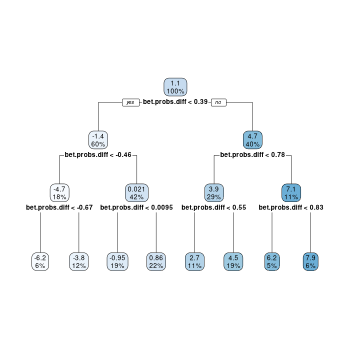
\includegraphics[width=\textwidth]{plots/handball-compromise-rpart-plot.png}
            \end{column}
            \begin{column}{0.6\textwidth}
                \newline
                \centering
                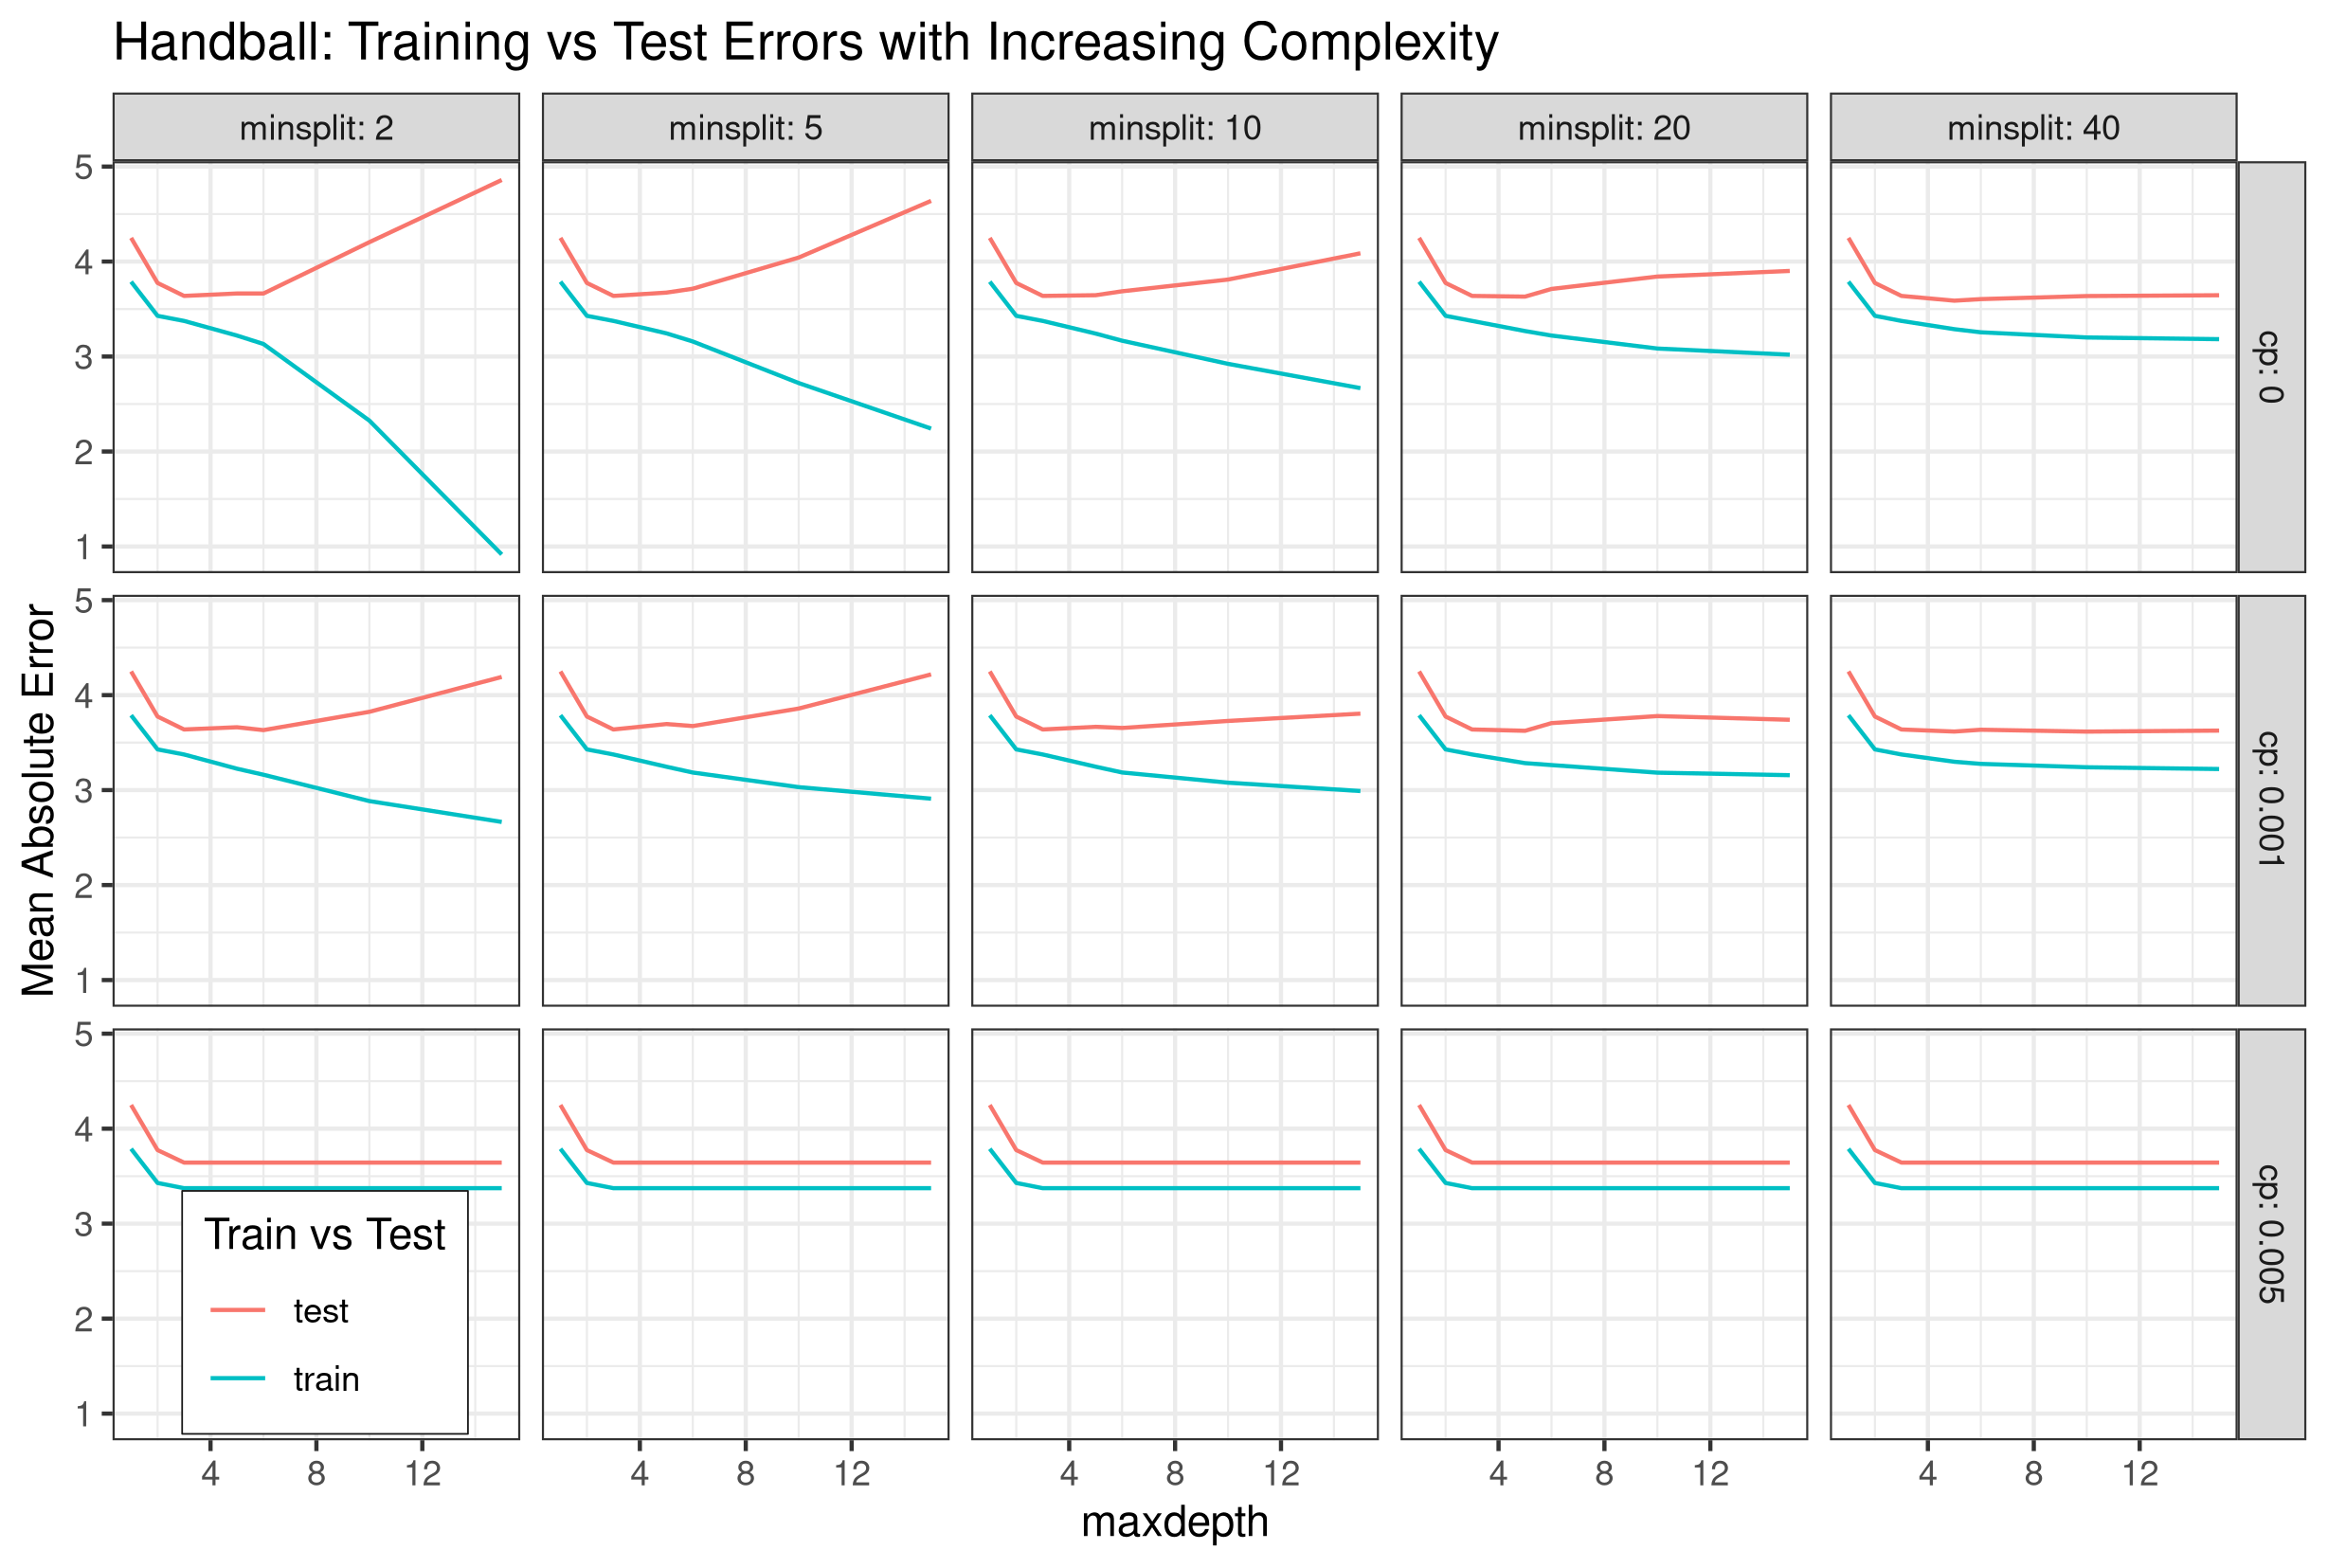
\includegraphics[width=\textwidth]{plots/handball-overfit-complexity-facet.png}
            \end{column}
        \end{columns}
    \end{frame}

    \begin{frame}
        \frametitle{Football Tree Regression}

        Highlight of Football Grid Search Model Comparison
        \newline
        \resizebox{\textwidth}{!} {
            \begin{tabular}{l|r|r|r|r|r|r|r|r}
            \hline
            comment & cp & minsplit & maxdepth & train\_mae & train\_rmse & test\_mae & test\_rmse & nsplits\\
            \hline
            best test mae & 0 & 5 & 3 & 0.780 & 0.980 & 0.741 & 0.985 & 7\\
            \hline
            a single split model does well & 0 & 2 & 1 & 0.835 & 1.064 & 0.770 & 1.041 & 1\\
            \hline
            worst overfit in mae \& rmse & 0 & 2 & 15 & 0.112 & 0.312 & 1.326 & 1.716 & 171\\
            \hline
            \end{tabular}
        }
        \newline
        \newline

        
        \begin{columns}[c]
            \begin{column}{0.36\textwidth}
                Best single split: 
                \centering
                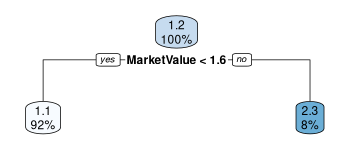
\includegraphics[height =.38\textwidth]{plots/football-one-split-rpart-plot.png}
                Lowest MAE: 
                
\includegraphics[width =\textwidth]{plots/football-best-rpart-plot.png}
            \end{column}
            \begin{column}{0.62\textwidth}
                \newline
                \centering
                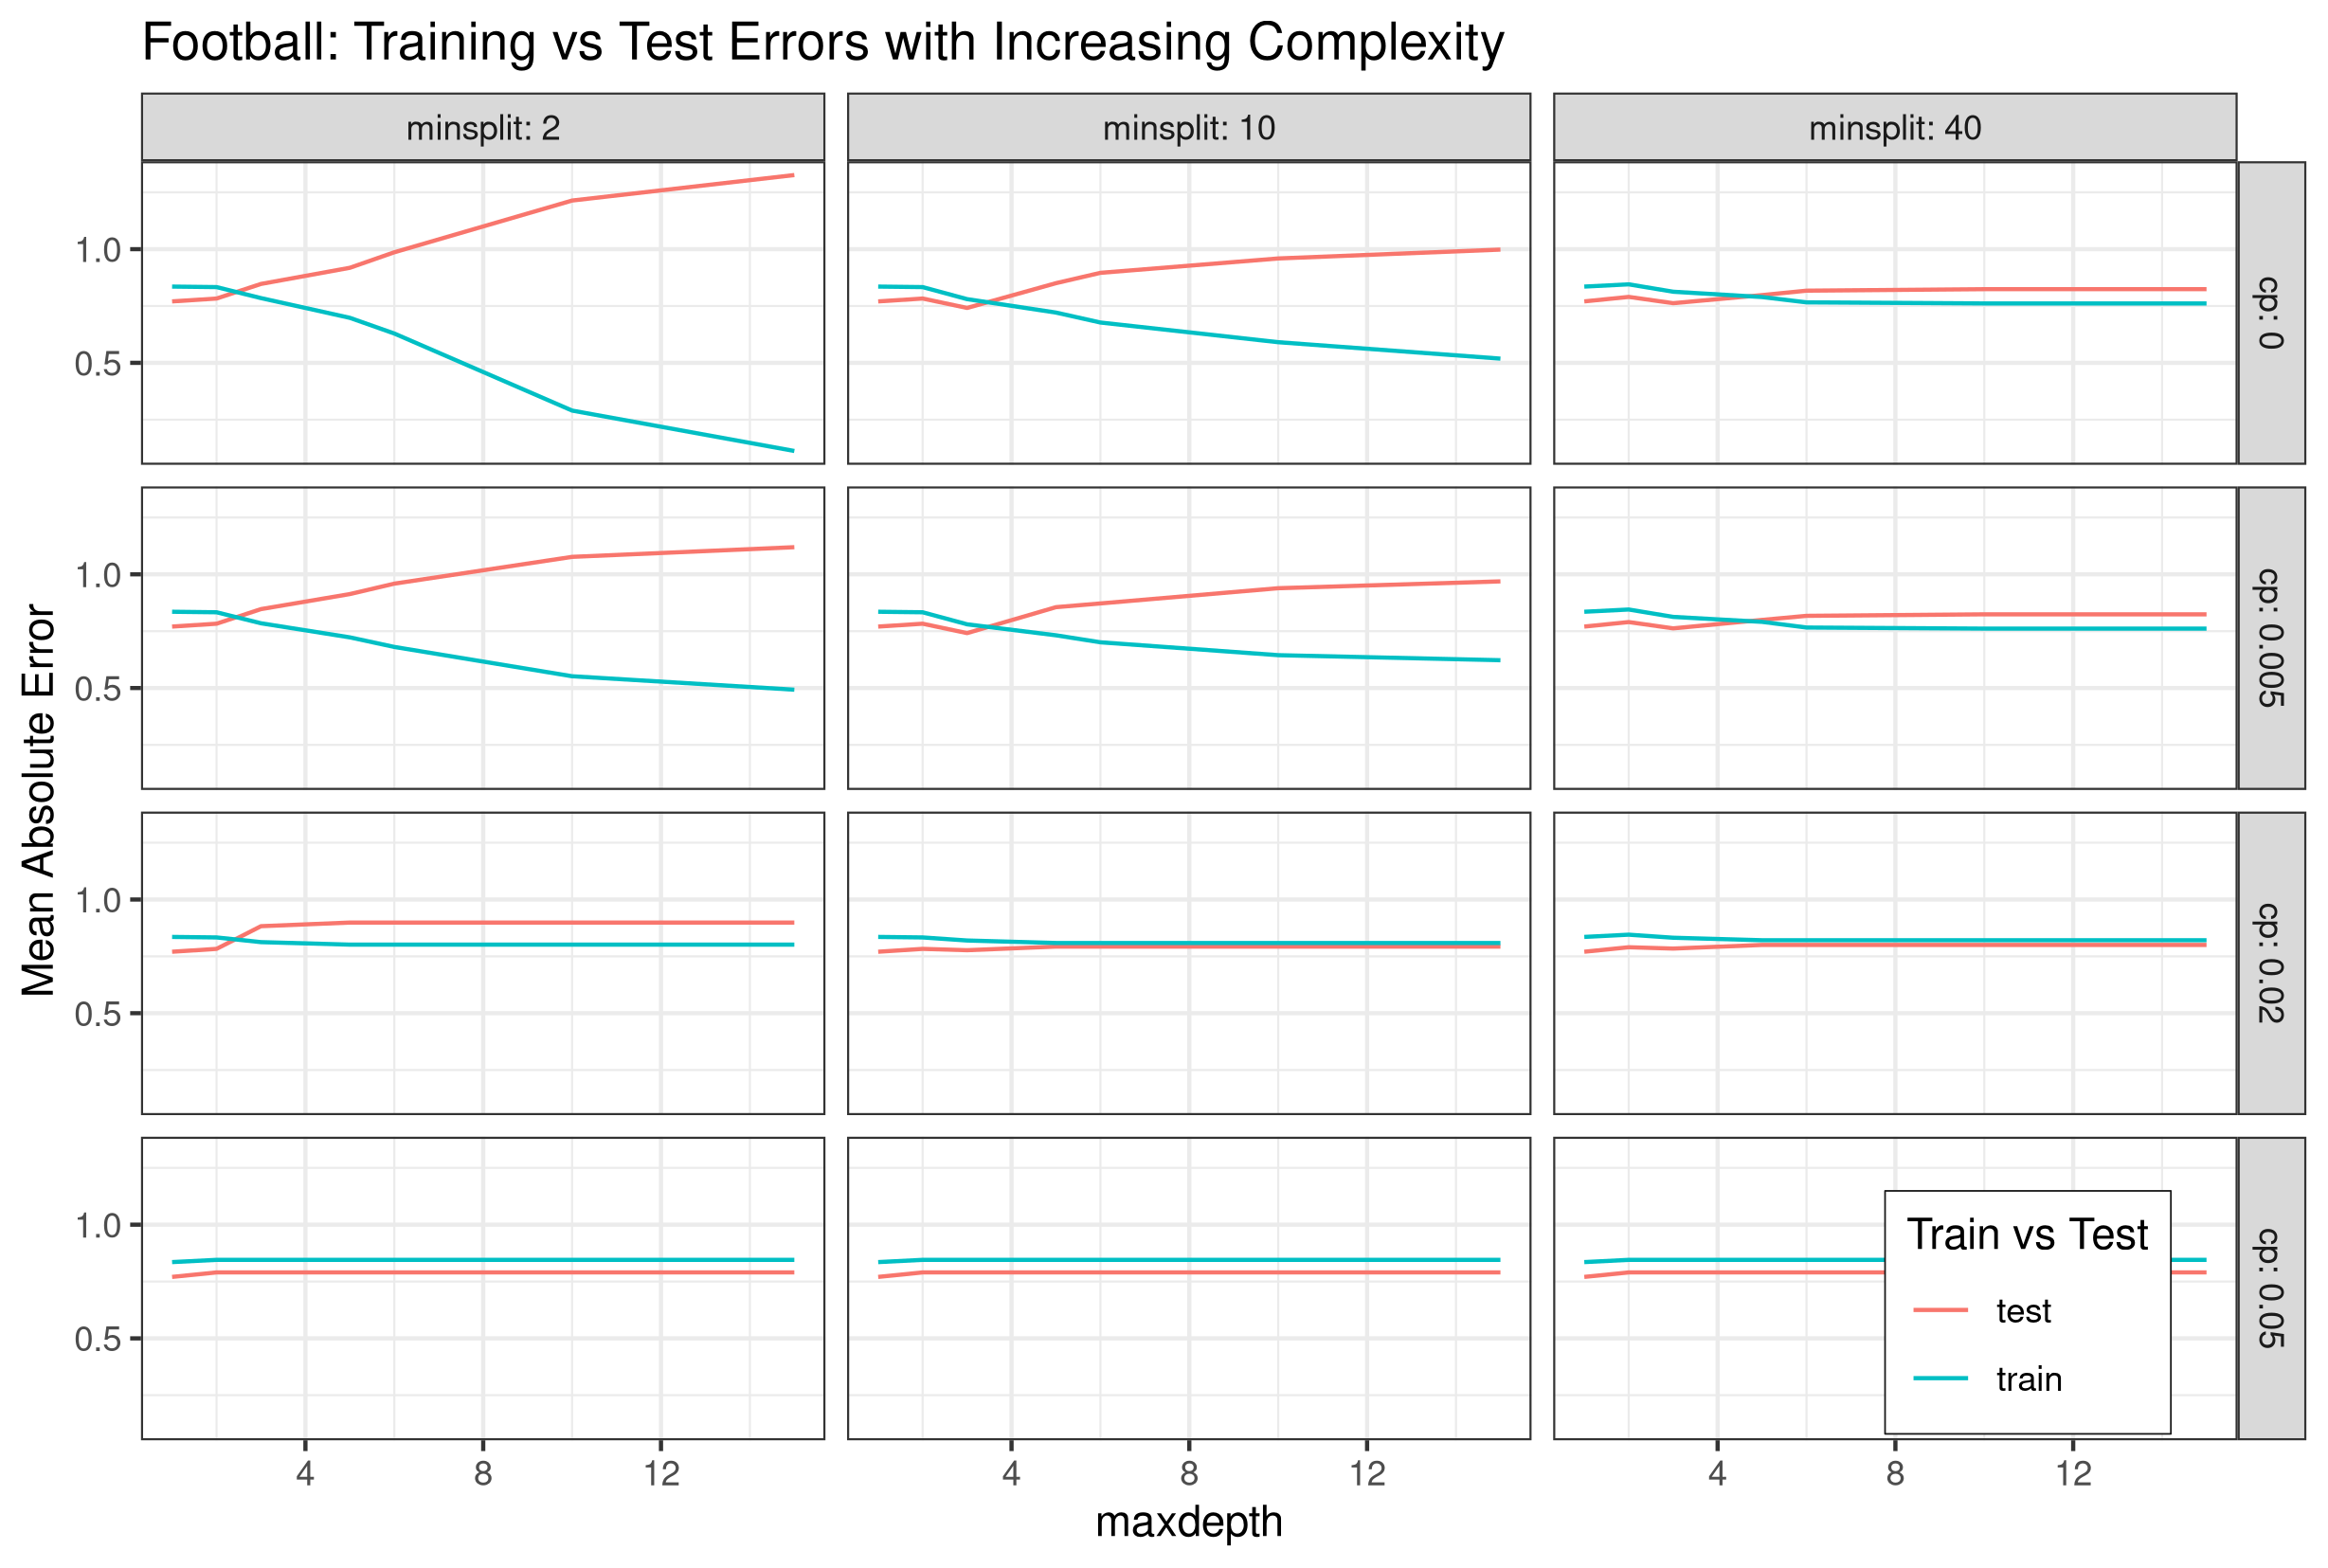
\includegraphics[width=\textwidth]{plots/football-overfit-complexity-facet.png}
            \end{column}
        \end{columns}
    \end{frame}

\end{document}